\section{Results}
\label{sec:results}

\subsection{Mesh Convergence}
\label{sec:mesh_convergence_results}

Table~\ref{tab:convergence_results} summarises the half-domain symmetry mesh convergence study. All three levels used the topoSet/subsetMesh cut approach (\S\ref{sec:symmetry}), 1500 simpleFoam iterations with $k$-$\omega$~SST, and force coefficients averaged over iterations 1000--1500.

\begin{table}[h]
    \centering
    \caption{Mesh convergence: half-domain symmetry results. $f = C_d + \tfrac{1}{3}C_l$.}
    \label{tab:convergence_results}
    \begin{tabular}{lcccccc}
        \toprule
        Level & Cells (half) & $C_d$ & $C_l$ & $f$ & Wall time (s) \\
        \midrule
        L1 (coarse)    & 182\,346  & 0.3569 & 0.1299 & 0.4001 & $\sim$120 \\
        L2 (medium)    & 435\,920  & 0.3302 & 0.2909 & 0.4271 & $\sim$260 \\
        L3 (fine)      & 912\,292  & 0.3249 & 0.3254 & 0.4334 & 627 \\
        \midrule
        Lienhart exp.\ & ---       & 0.299  & ---    & ---    & --- \\
        \bottomrule
    \end{tabular}
\end{table}

$C_d$ decreases monotonically from L1 to L3; the 1.6\% L2--L3 change confirms near mesh-convergence for $C_d$ at L3. However, $C_l$ continues to rise with refinement (12\% L2--L3 change) and no L4 data is available (L4 diverged). A residual L3--$L_\infty$ $C_l$ error of $\pm0.05$ would shift $f_1$ by $\pm0.017$ — comparable to the claimed MF improvement — so all absolute $f_1$ comparisons in this study are made on a consistent mesh (L3 vs L3) rather than against a mesh-converged reference. The DoE campaign uses L2 for efficiency ($\sim$260\,s/case at 8 cores).

\subsection{Symmetry Validation}
\label{sec:symmetry_validation}

The L2 symmetry mesh ($C_d = 0.3302$) agrees with the L2 full-domain result ($C_d = 0.330$) to within 0.6\%, confirming that the topoSet/subsetMesh half-plane approach introduces negligible error.

\subsection{Phase 1 DoE — Sobol Sensitivity Analysis}
\label{sec:sobol_results}

A 30-point Phase~1 LHS was evaluated across the four design variables ($\alpha_\mathrm{slant}$, $\alpha_\mathrm{diff}$, $h$, $R_\mathrm{nose}$). Total solve time was approximately 100~minutes at 8 cores (Mac Mini M4 Pro), averaging $\approx$200~s per case. Cd ranged from 0.263 to 0.580 and the objective $f = C_d + \tfrac{1}{3}C_l$ from 0.178 to 0.819.

Sobol total-order sensitivity indices computed from the GP surrogate are shown in Table~\ref{tab:sobol}. Slant angle and diffuser angle together account for nearly all of the variance in $f$ (each $S_T > 0.7$), confirming that these are the dominant design levers. The large gap between $S_1$ and $S_T$ for both variables indicates strong nonlinear interaction between slant and diffuser angles.

\begin{table}[h]
    \centering
    \caption{Sobol sensitivity indices for $f = C_d + \tfrac{1}{3}C_l$ from Phase~1 GP surrogate ($N=2048$ Saltelli sample, 20\,480 GP evaluations).}
    \label{tab:sobol}
    \begin{tabular}{lcccc}
        \toprule
        Variable & $S_1$ & $S_T$ & $S_T$ conf.\ & Classification \\
        \midrule
        Slant angle $\alpha_\mathrm{slant}$   & 0.217 & 0.759 & $\pm$0.064 & Strong \\
        Diffuser angle $\alpha_\mathrm{diff}$ & 0.144 & 0.713 & $\pm$0.073 & Strong \\
        Ride height $h$                        & 0.025 & 0.096 & $\pm$0.009 & Moderate \\
        Nose radius $R_\mathrm{nose}$          & 0.000 & 0.001 & $\pm$0.000 & Weak — eliminated \\
        \bottomrule
    \end{tabular}
\end{table}

$R_\mathrm{nose}$ ($S_T = 0.001$) is eliminated from the design space; $h$ ($S_T = 0.096$) is fixed at the Lienhart nominal value $h = 50.8$~mm, as its moderate influence does not justify the additional DoE dimensionality. Both are fixed at their default values for Phase~2.

\begin{figure}[h]
  \centering
  \pgffig{0.62\textwidth}{residuals_optimum}
  \caption{simpleFoam residual convergence for the optimum design (case~021, L2 mesh). The shaded band marks the 600--800 iteration averaging window used for force-coefficient extraction. All residuals reach below $10^{-4}$ by iteration 300.}
  \label{fig:residuals}
\end{figure}

\begin{figure}[h]
  \centering
  \pgffig{0.62\textwidth}{forcecoeffs_optimum}
  \caption{$C_d$ and $C_l$ iteration history for the optimum design (case~021). Shaded region indicates the averaging window (iterations 600--800). Both coefficients are stationary well before averaging begins.}
  \label{fig:forcecoeffs}
\end{figure}

\paragraph{Phase 1 GP accuracy.} Leave-one-out cross-validation on the 30-point Phase~1 data gives $R^2 = -0.21$ for $C_d$ and $R^2 = -0.50$ for $C_l$. Negative $R^2$ reflects the sparsity of 30 points in a 4-D space, and motivates the reduction to 2 active variables and a denser Phase~2 sweep. The Sobol indices are nonetheless qualitatively reliable given the clear separation in $S_T$ magnitudes.

% ----------------------------------------------------------------
\subsection{Phase 2 DoE — Dense Two-Variable Sweep}
\label{sec:doe_phase2}

With $R_\mathrm{nose}$ and $h$ fixed, a 50-point LHS was generated over the two active variables:
\[
  \alpha_\mathrm{slant} \in [15^\circ, 40^\circ], \quad
  \alpha_\mathrm{diff}  \in [0^\circ,  20^\circ].
\]
The centred $L_2$-discrepancy of the selected sample (best of 10 LHS candidates) was 0.000478. All 50 simpleFoam cases converged successfully on the L2 mesh ($\sim$435\,K cells, 8 cores, $\sim$200~s/case). The objective ranged from $f = 0.178$ to $f = 0.819$ across the design space. Figure~\ref{fig:doe_scatter} shows the distribution of all 50 CFD evaluations in the design space, coloured by objective value. The best Phase~2 DoE point was case~021:
\[
  \alpha_\mathrm{slant} = 32.5^\circ,\quad
  \alpha_\mathrm{diff}  = 8.9^\circ,\quad
  C_d = 0.3187,\quad C_l = -0.3274,\quad f = 0.2096.
\]

\begin{figure}[h]
  \centering
  \pgffig{0.58\textwidth}{doe_scatter}
  \caption{Phase~2 DoE design space. Each point is one simpleFoam evaluation; colour indicates the objective $f = C_d + \tfrac{1}{3}C_l$. The red star marks the DoE best (case~021).}
  \label{fig:doe_scatter}
\end{figure}

% ----------------------------------------------------------------
\subsection{GP Surrogate — Phase 2 Accuracy}
\label{sec:gp_phase2}

Separate GP regressors were fitted to $C_d$ and $C_l$ using a Mat\'{e}rn-$5/2$ ARD kernel plus a white-noise term. Fitted kernels:

\begin{align*}
  k_{C_d} &= 1.04^2 \cdot \mathrm{Mat\acute{e}rn}_{5/2}(\ell = [1.02,\,0.30]) + \sigma^2_n = 0.074 \\
  k_{C_l} &= 0.98^2 \cdot \mathrm{Mat\acute{e}rn}_{5/2}(\ell = [0.66,\,0.26]) + \sigma^2_n = 0.100
\end{align*}

Leave-one-out cross-validation on the 50 Phase~2 CFD points gives $R^2 = 0.627$ ($\mathrm{MAE} = 0.013$) for $C_d$ and $R^2 = 0.417$ ($\mathrm{MAE} = 0.096$) for $C_l$ (Figure~\ref{fig:gp_validation}). Both are a substantial improvement over the Phase~1 model, confirming that the 50-point 2-D sweep yields a useful predictive surface.

\begin{figure}[h]
  \centering
  \pgffig{0.75\textwidth}{gp_validation}
  \caption{GP leave-one-out cross-validation for Phase~2. Left: $C_d$ ($R^2=0.627$). Right: $C_l$ ($R^2=0.417$). Dashed line is perfect prediction.}
  \label{fig:gp_validation}
\end{figure}

\paragraph{Phase 2 Sobol analysis.} Sobol total-order sensitivity indices re-evaluated on the Phase~2 GP surrogate are shown in Table~\ref{tab:sobol_phase2}. Diffuser angle emerges as the dominant variable for $f$ ($S_T = 0.725$), with slant angle contributing strongly ($S_T = 0.499$). No variable can be eliminated at this stage.

\begin{table}[h]
  \centering
  \caption{Phase~2 Sobol total-order sensitivity indices ($N=2048$ Saltelli sample).}
  \label{tab:sobol_phase2}
  \begin{tabular}{lccccc}
    \toprule
    Variable & \multicolumn{2}{c}{$C_d$} & \multicolumn{2}{c}{$C_l$} & \multicolumn{1}{c}{$f$} \\
    \cmidrule(lr){2-3}\cmidrule(lr){4-5}\cmidrule(lr){6-6}
     & $S_1$ & $S_T$ & $S_1$ & $S_T$ & $S_T$ \\
    \midrule
    Slant angle $\alpha_\mathrm{slant}$   & 0.299 & 0.500$\pm$0.043 & 0.465 & 0.678$\pm$0.052 & 0.499$\pm$0.039 \\
    Diffuser angle $\alpha_\mathrm{diff}$ & 0.505 & 0.707$\pm$0.047 & 0.317 & 0.529$\pm$0.042 & 0.725$\pm$0.050 \\
    \bottomrule
  \end{tabular}
\end{table}

\paragraph{Surrogate optimum.} Single-objective minimisation of $f = C_d + \tfrac{1}{3}C_l$ on the GP mean surface (Nelder--Mead, 5000 random restarts) yields:
\[
  \alpha_\mathrm{slant}^* = 33.9^\circ,\quad
  \alpha_\mathrm{diff}^*  = 9.08^\circ,\quad
  \hat{C}_d = 0.3153,\quad \hat{C}_l = -0.3175,\quad \hat{f} = 0.2094.
\]
This surrogate prediction is consistent with the CFD-observed DoE best ($f=0.2096$), validating the GP model in the optimum region.

\begin{figure}[h]
  \centering
  \pgffig{0.95\textwidth}{response_surfaces}
  \caption{GP response surface for $f = C_d + \tfrac{1}{3}C_l$ over the Phase~2 design space. The black cross marks the surrogate optimum ($\alpha_\mathrm{slant}=33.9^\circ$, $\alpha_\mathrm{diff}=9.08^\circ$). The star marks the CFD best DoE point (case~021).}
  \label{fig:response_surface}
\end{figure}

\paragraph{Pareto front.} Multi-objective Pareto optimisation (minimise $C_d$, maximise downforce $-C_l$) on the GP surface identifies 61 non-dominated designs. The front extremes are:
\begin{itemize}
  \item \emph{Minimum drag:} $\alpha_\mathrm{slant}=15.3^\circ$, $\alpha_\mathrm{diff}=9.6^\circ$, $\hat{C}_d=0.277$, $\hat{C}_l=-0.014$ (near-zero downforce).
  \item \emph{Maximum downforce:} $\alpha_\mathrm{slant}=33.8^\circ$, $\alpha_\mathrm{diff}=9.1^\circ$, $\hat{C}_d=0.316$, $\hat{C}_l=-0.318$ (14\% drag penalty for maximum downforce).
\end{itemize}

\begin{figure}[h]
  \centering
  \pgffig{0.72\textwidth}{campaign_convergence}
  \caption{Objective $f$ across all 100 CFD evaluations in the optimisation campaign (30 Phase~1 + 50 Phase~2 + 20 BO). The solid line is the running best. Vertical dashed lines mark phase boundaries.}
  \label{fig:campaign}
\end{figure}

% ----------------------------------------------------------------
\subsection{Bayesian Optimisation}
\label{sec:bo_results}

Twenty Bayesian Optimisation (BO) iterations were performed using Expected Improvement (EI) acquisition. At each iteration the acquisition function was maximised over the Phase~2 bounds, a full CFD case was run on the L2 mesh, and the GP was updated with the new observation. The run used 8 cores per case ($\sim$200~s/solve) for a total BO wall time of approximately 70~minutes.

\begin{figure}[h]
  \centering
  \pgffig{0.75\textwidth}{bo_convergence}
  \caption{BO convergence history. Upper panel: CFD objective $f_\mathrm{cfd}$ per iteration (dots) and running best $f$ (solid line). Lower panel: maximum Expected Improvement (EI) at each iteration. The horizontal dashed line indicates the Phase~2 DoE best ($f=0.2096$).}
  \label{fig:bo_convergence}
\end{figure}

The running best $f$ remained at the Phase~2 DoE incumbent of $f = 0.2096$ throughout all 20 BO iterations — no BO point improved on the DoE best. Selected iteration results are shown in Table~\ref{tab:bo_iterations}.

\begin{table}[h]
  \centering
  \caption{Selected Bayesian Optimisation iterations. $f_\mathrm{pred}$ is the GP mean prediction; $f_\mathrm{cfd}$ is the CFD result. EI is the maximum Expected Improvement at the time of selection.}
  \label{tab:bo_iterations}
  \begin{tabular}{ccccccc}
    \toprule
    Iter & $\alpha_\mathrm{slant}$ (°) & $\alpha_\mathrm{diff}$ (°) & $f_\mathrm{pred}$ & EI & $C_{d,\mathrm{cfd}}$ & $f_\mathrm{cfd}$ \\
    \midrule
     1 & 35.7 &  9.31 & 0.2108 & 0.01550 & 0.487 & 0.642 \\
     2 & 31.7 &  8.79 & 0.2039 & 0.01591 & 0.307 & 0.275 \\
    10 & 38.9 &  5.58 & 0.2630 & 0.00556 & 0.295 & 0.228 \\
    19 & 37.6 &  3.34 & 0.2229 & 0.01113 & 0.301 & 0.237 \\
    20 & 32.8 &  9.54 & 0.2474 & 0.00833 & 0.308 & 0.303 \\
    \midrule
    \multicolumn{4}{l}{DoE best (case~021)} & --- & 0.319 & \textbf{0.2096} \\
    \bottomrule
  \end{tabular}
\end{table}

The EI decreased from 0.0155 at iteration~1 to $\approx$0.005--0.008 by iteration~20 but did not reach the convergence threshold of $10^{-4}$, indicating residual GP uncertainty in unexplored high-slant, low-diffuser regions. The lowest individual $C_d$ achieved by BO was 0.295 (iteration~10: $\alpha_\mathrm{slant}=38.9^\circ$, $\alpha_\mathrm{diff}=5.6^\circ$), but the associated $C_l = -0.200$ gives $f = 0.228$, worse than the DoE incumbent on the combined objective.

\paragraph{Interpretation.} The BO failure to improve on the DoE incumbent is consistent with the GP response surface: the minimum of $f$ lies in a narrow ridge near $\alpha_\mathrm{slant}\approx32$--$34^\circ$, $\alpha_\mathrm{diff}\approx9^\circ$. The Phase~2 DoE already sampled this region (case~021), and the GP surrogate correctly identified it as near-optimal. Iteration~1's large over-prediction error ($f_\mathrm{pred}=0.211$ vs.\ $f_\mathrm{cfd}=0.642$ at $35.7^\circ/9.3^\circ$) was identified as a pseudo-time limit-cycle artefact rather than a physical design penalty: the mesh quality was verified to be equivalent to converged cases, but the force history exhibits $\sigma_{C_d}=0.023$ over the averaging window, indicating an oscillating RANS state (see \S\ref{sec:des_statistics}). A subsequent L3 re-solve of this geometry returns $C_d=0.295$, $f_1=0.215$ with $\sigma_{C_d}=0.002$ — a well-converged, physically plausible value (\S\ref{sec:stencil}). The L2 training value of $f=0.642$ therefore inflates GP uncertainty in the transition region ($\alpha_\mathrm{slant}\approx33$--$37^\circ$) and biased the BO acquisition function away from the high-slant basin where the true MF optimum resides.

% ----------------------------------------------------------------
\subsection{Summary of Optimal Design}
\label{sec:optimum_summary}

The single-fidelity L2 optimum is the Phase~2 DoE best (case~021, Table~\ref{tab:optimum_l2}). This result motivated the multi-fidelity correction described in \S\ref{sec:mf_results}, which relocates the optimum after accounting for the L2--L3 fidelity gap. The MF-corrected final optimum is reported in Table~\ref{tab:mf_optimum}.

\begin{table}[h]
  \centering
  \caption{L2 single-fidelity optimal Ahmed body design (baseline for MF correction).}
  \label{tab:optimum_l2}
  \begin{tabular}{lc}
    \toprule
    Parameter & Value \\
    \midrule
    Slant angle $\alpha_\mathrm{slant}$ & $32.5^\circ$ \\
    Diffuser angle $\alpha_\mathrm{diff}$ & $8.9^\circ$ \\
    Ride height $h$                       & $50.8$~mm (fixed) \\
    Nose radius $R_\mathrm{nose}$         & $100$~mm (fixed) \\
    \midrule
    $C_d$ (L2 RANS)   & 0.3187 \\
    $C_l$ (L2 RANS)   & $-$0.3274 \\
    $f = C_d + \tfrac{1}{3}C_l$ & 0.2096 \\
    \midrule
    Lienhart baseline ($25^\circ$ slant) & $C_d = 0.299$ \\
    \bottomrule
  \end{tabular}
\end{table}

The L2 optimum at $32.5^\circ$ lies above the Lienhart baseline ($25^\circ$), where stronger slant vortices generate meaningful downforce ($C_l = -0.327$) at a modest drag cost ($C_d = 0.319$ vs.\ 0.299 baseline). However, as shown in \S\ref{sec:l3_validation}, the L3 mesh predicts substantially less downforce at this point ($\Delta C_l = +0.160$), motivating the MF co-Kriging correction. The MF analysis relocates the final optimum to $\alpha_\mathrm{slant}=38.9^\circ$, $\alpha_\mathrm{diff}=10.5^\circ$ (Table~\ref{tab:mf_optimum}).

\begin{figure}[h]
  \centering
  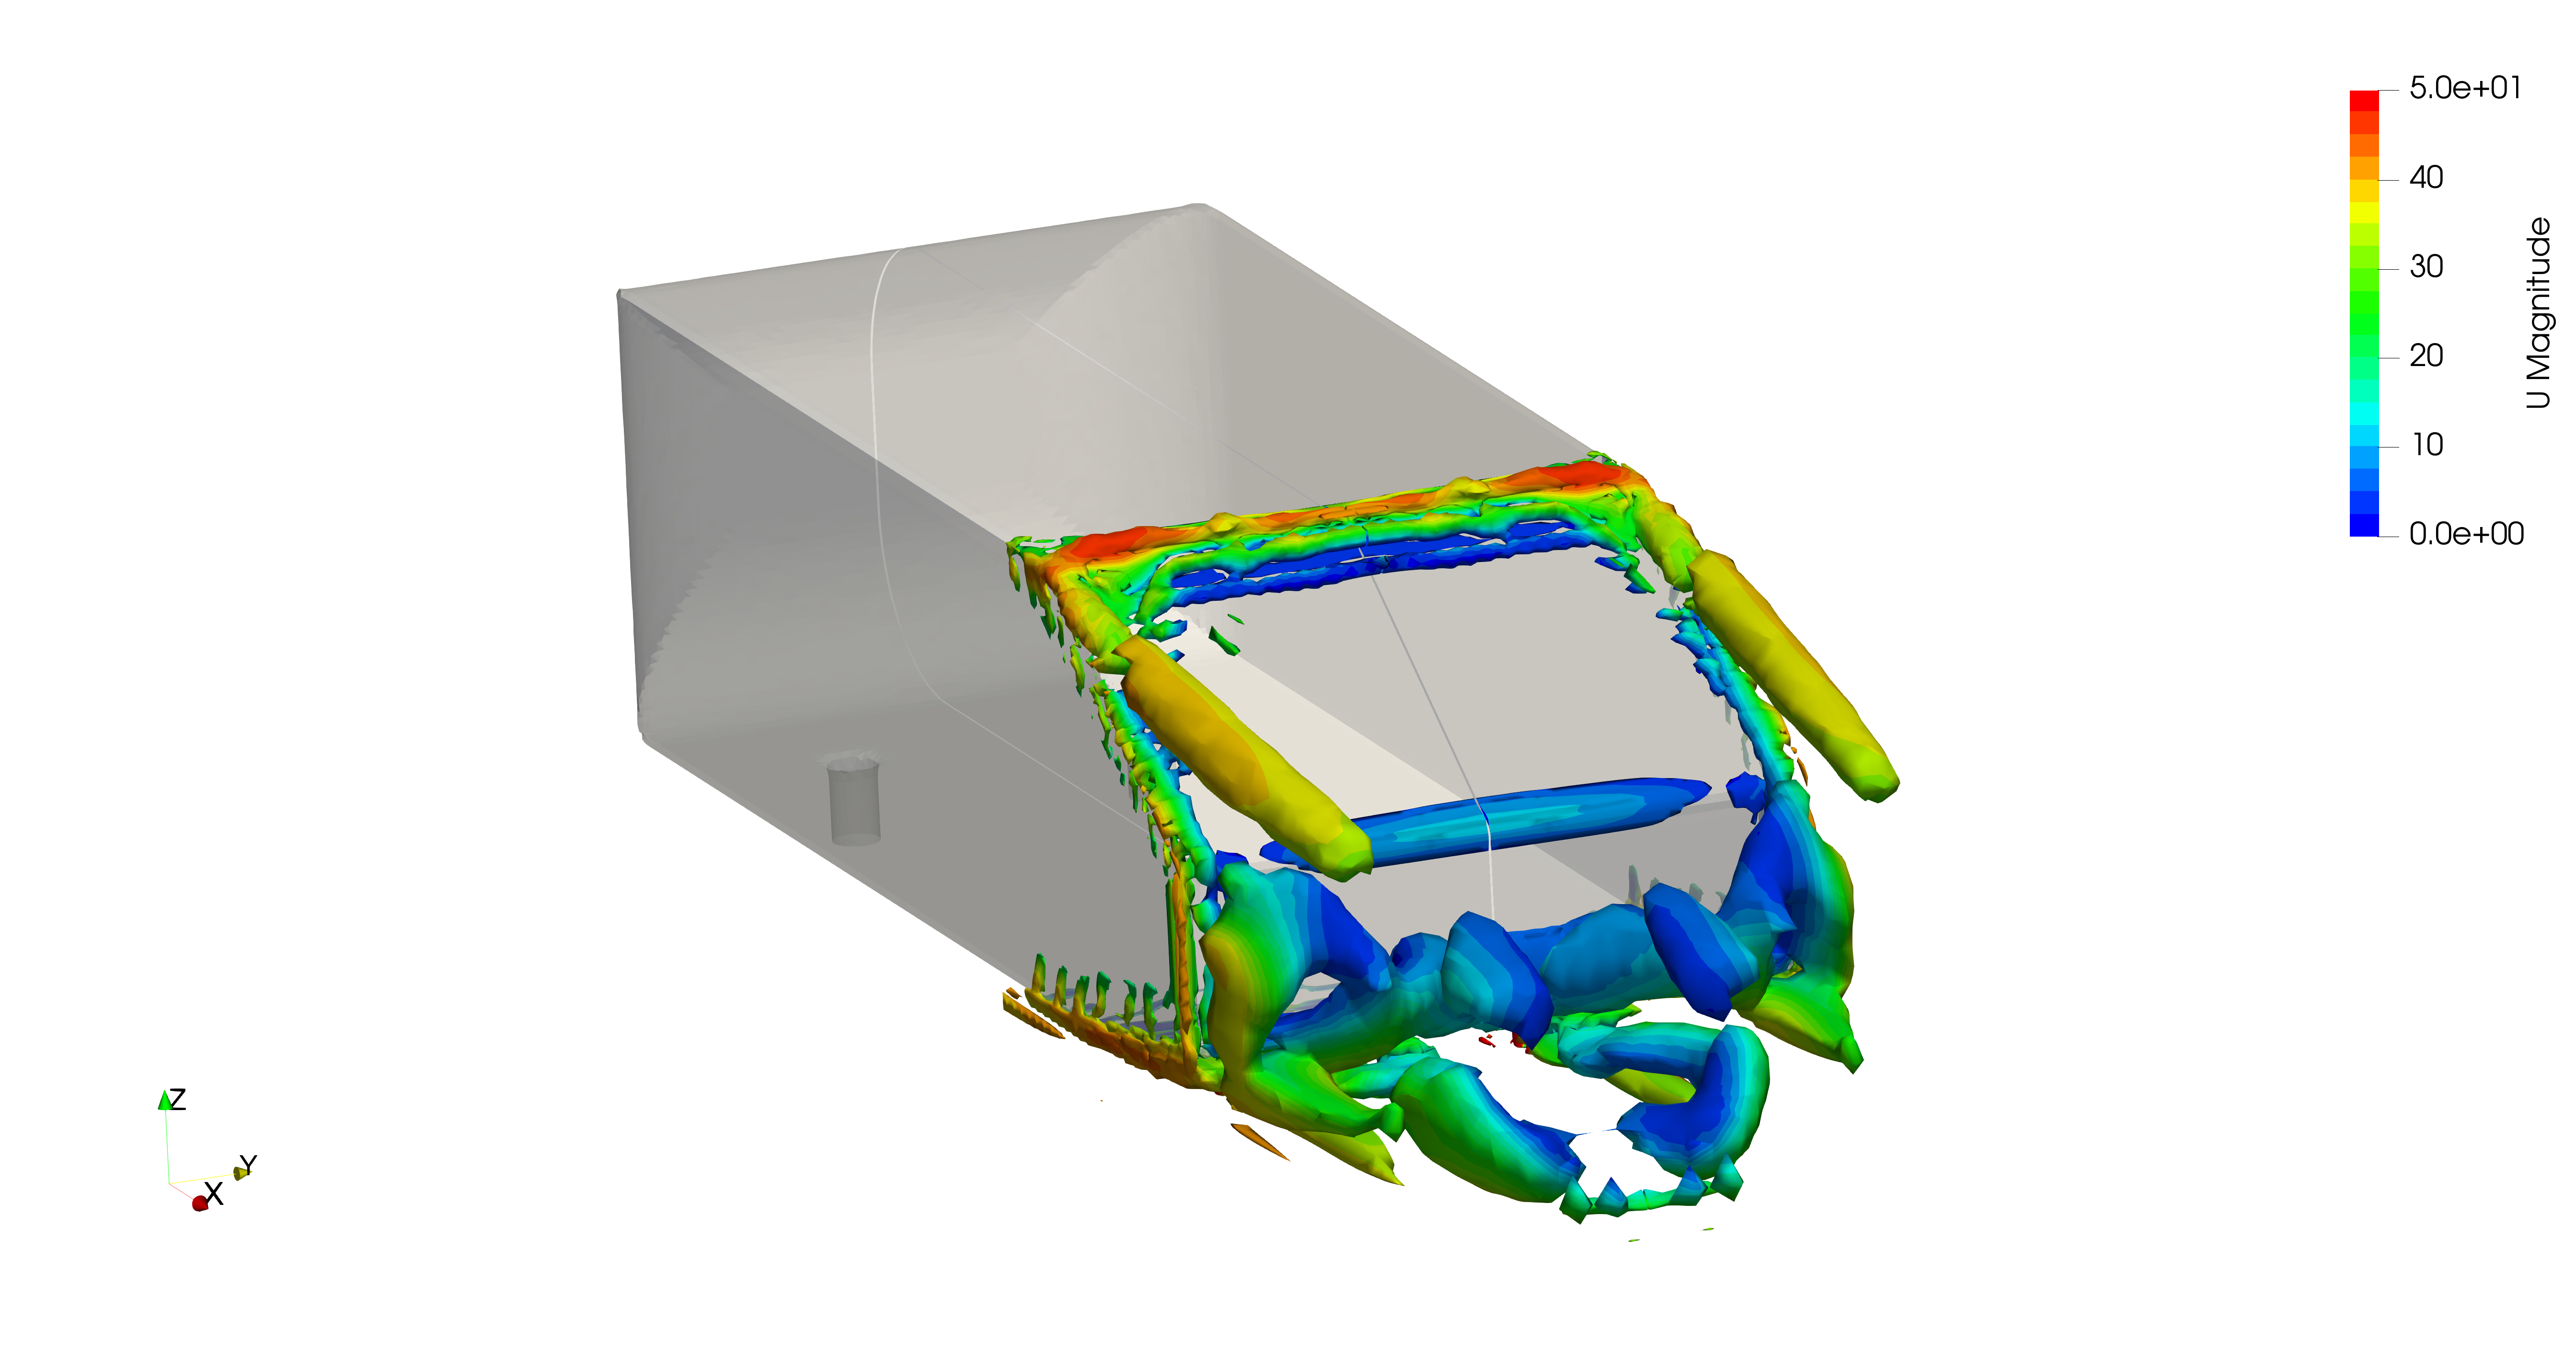
\includegraphics[width=0.95\textwidth]{figures/q_criterion_optimum}
  \caption{Q-criterion isosurface coloured by velocity magnitude at the optimum design ($\alpha_\mathrm{slant}=32.5^\circ$, $\alpha_\mathrm{diff}=8.9^\circ$, L2 mesh, $Q = 20{,}000$~s$^{-2}$). The two C-pillar vortex cores originate at the slant side edges and trail into the wake; the central low-speed region on the slant face indicates surface separation consistent with the above-critical-angle flow regime. These structures are responsible for the predicted $C_l = -0.327$ downforce.}
  \label{fig:q_criterion}
\end{figure}

\begin{figure}[h]
  \centering
  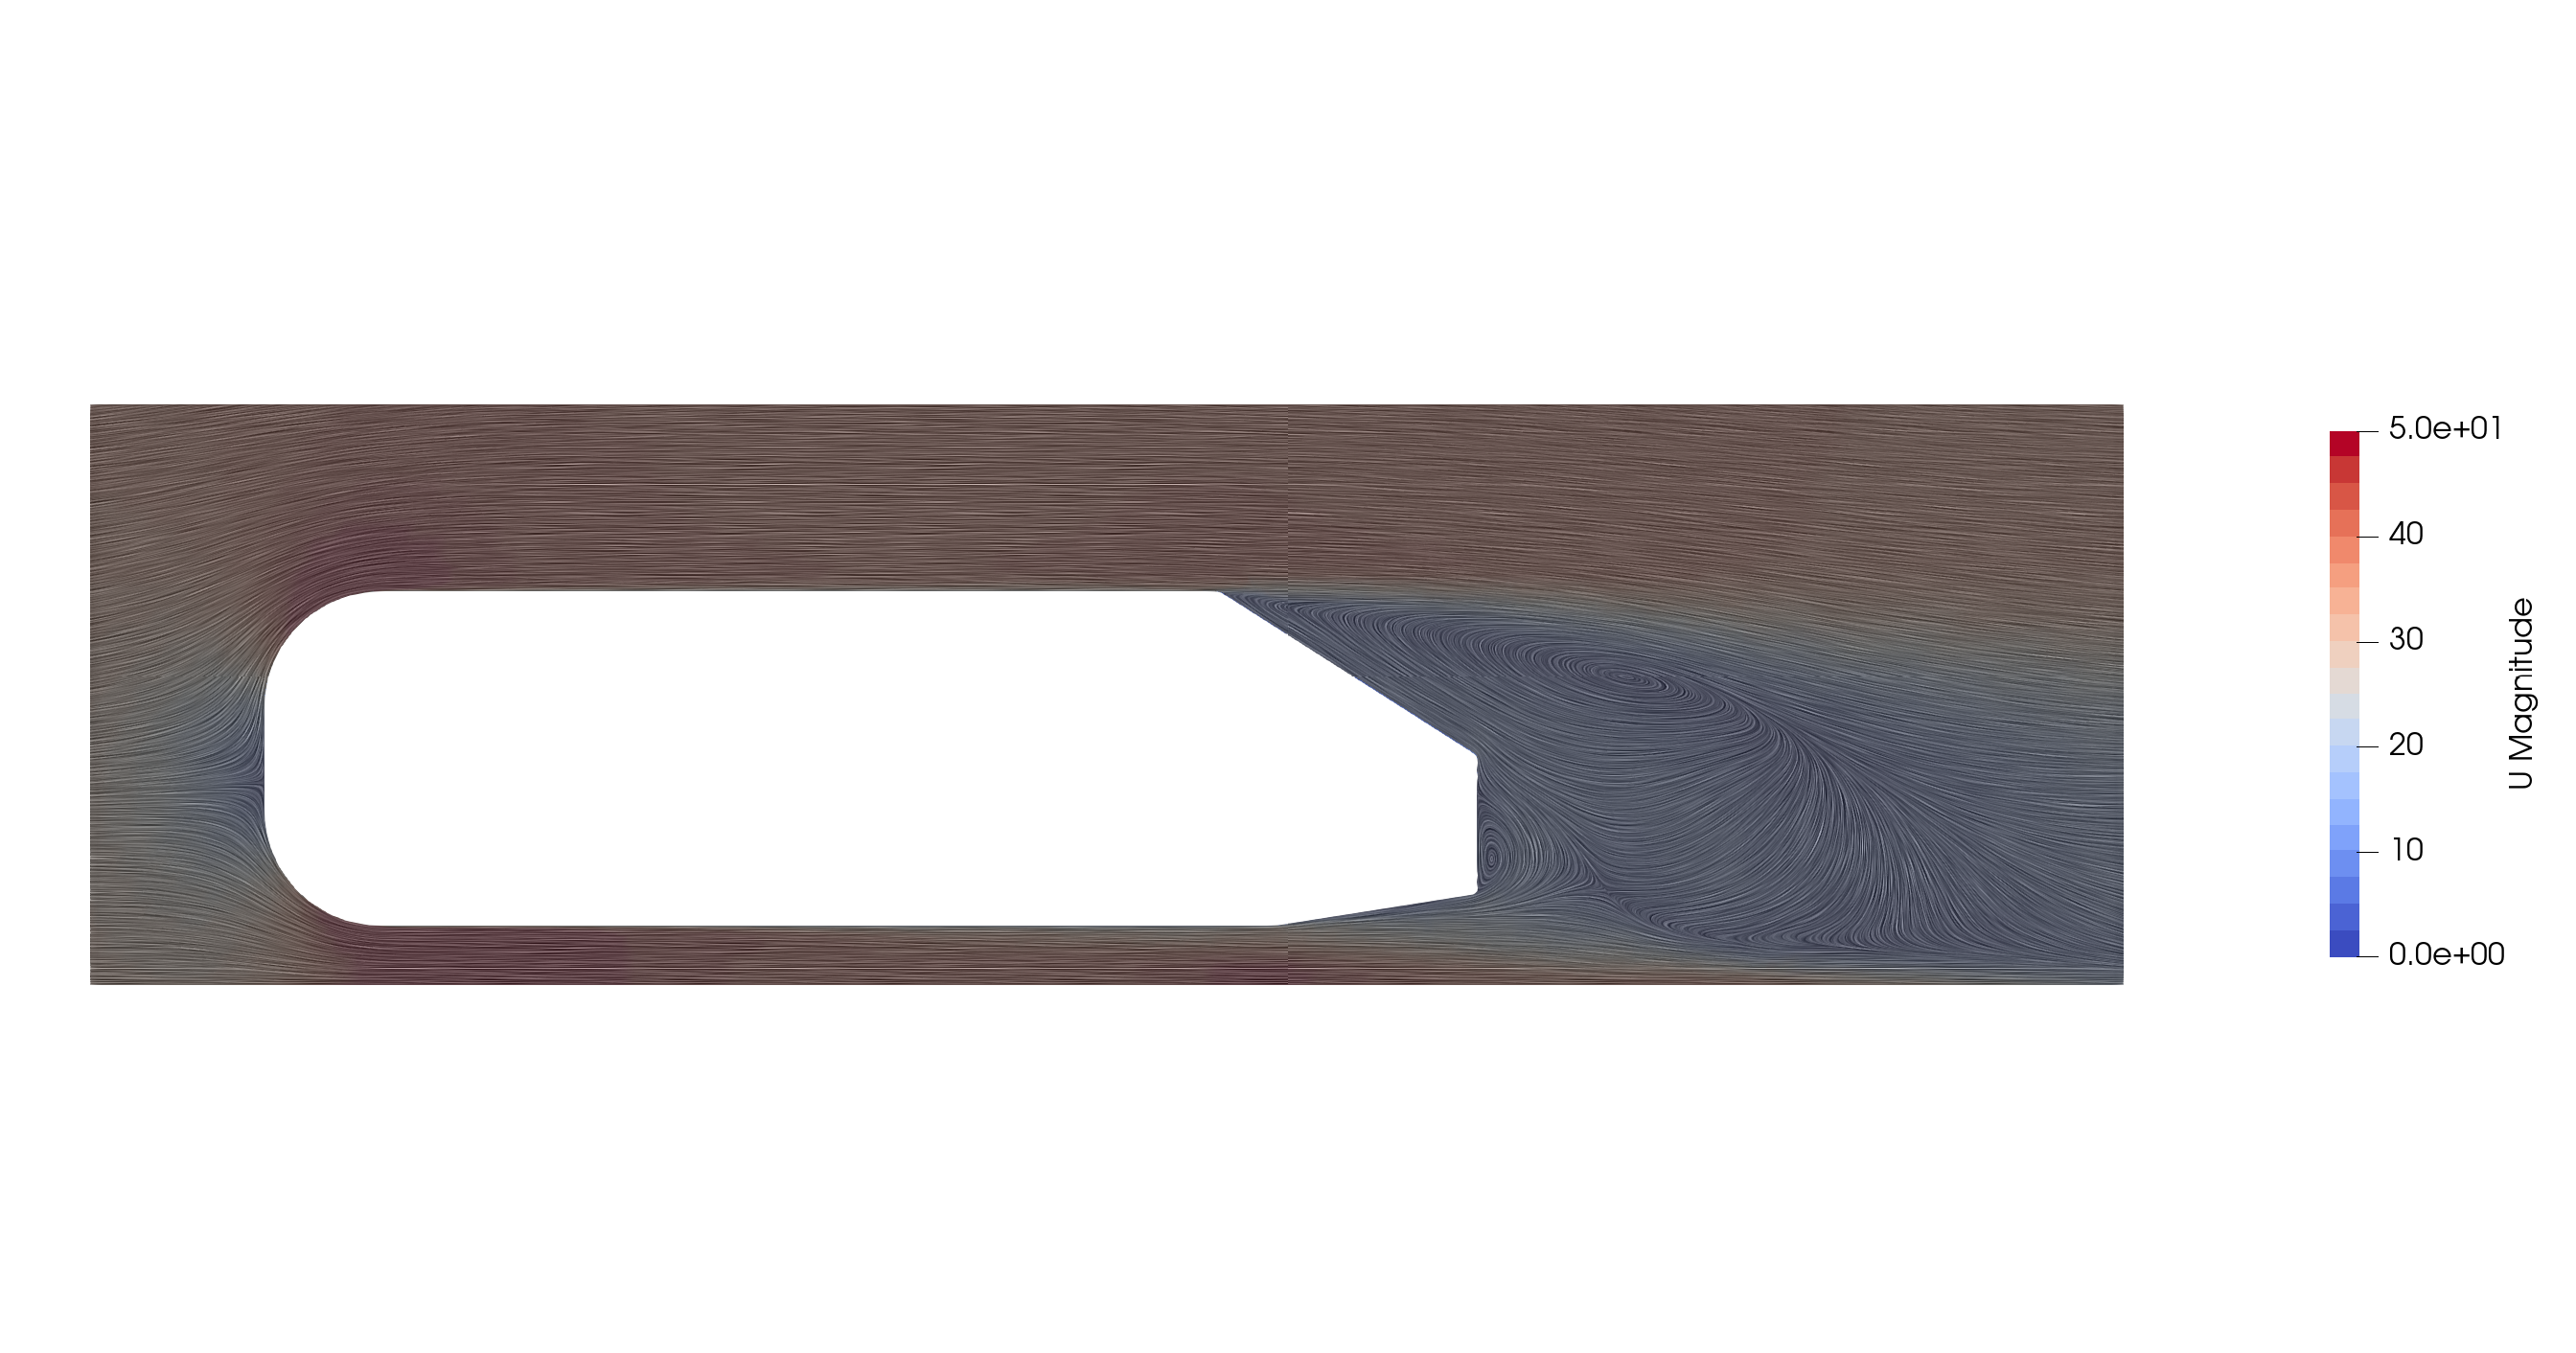
\includegraphics[width=0.95\textwidth]{figures/symmetry_plane_lic}
  \caption{Surface LIC on the symmetry plane ($y=0$) coloured by velocity magnitude at the optimum design (L2 mesh, $U_\infty = 40$~m/s). Flow is left to right. Attached acceleration over the nose and roof is visible; the slant surface shows a recirculation pattern consistent with separated flow above the critical slant angle; the large spiral structure behind the base is the wake recirculation bubble.}
  \label{fig:symmetry_lic}
\end{figure}

% ----------------------------------------------------------------
\subsection{L3 Fine-Mesh Validation at the Optimum}
\label{sec:l3_validation}

To assess fidelity-level sensitivity, the confirmed optimum design ($\alpha_\mathrm{slant}=32.5^\circ$, $\alpha_\mathrm{diff}=8.9^\circ$) was re-evaluated on the L3 fine mesh ($\sim$912\,K half-domain cells, 4 boundary layers, maxCellSize 0.133~m) using identical solver settings. Results are compared with the L2 DoE result in Table~\ref{tab:l3_validation}.

\begin{table}[h]
  \centering
  \caption{L2 vs L3 mesh comparison at the optimum design point.}
  \label{tab:l3_validation}
  \begin{tabular}{lcccc}
    \toprule
    Mesh & Cells (half) & $C_d$ & $C_l$ & $f$ \\
    \midrule
    L2 medium (DoE, case~021) & 435\,920  & 0.3187 & $-$0.3274 & 0.2096 \\
    L3 fine   (validation)    & 912\,292  & 0.3032 & $-$0.1670 & 0.2475 \\
    \midrule
    Difference                & ---        & $-$0.015 & $+$0.160  & $+$0.038 \\
    \bottomrule
  \end{tabular}
\end{table}

The L3 mesh predicts 4.9\% lower $C_d$ (0.303 vs.\ 0.319) but substantially less downforce: $C_l = -0.167$ vs.\ $-0.327$ on L2. This discrepancy is physically significant. On the coarser L2 grid the slant boundary layer is under-resolved, and the onset of separation is likely delayed — yielding an artificially strong trailing vortex system and higher downforce. The L3 mesh, with a finer near-wall layer ($\Delta y_\mathrm{first} = 3.5\times10^{-2}$~m vs.\ $5\times10^{-2}$~m) and 4 BL layers, better captures the adverse pressure gradient on the slant and predicts earlier or more extensive separation. The resulting $f = 0.248$ on L3 is 18\% higher than the L2 estimate; this mesh-sensitivity warrants noting as a limitation of the L2-based optimisation campaign.

\begin{figure}[h]
  \centering
  \begin{subfigure}[b]{0.48\textwidth}
    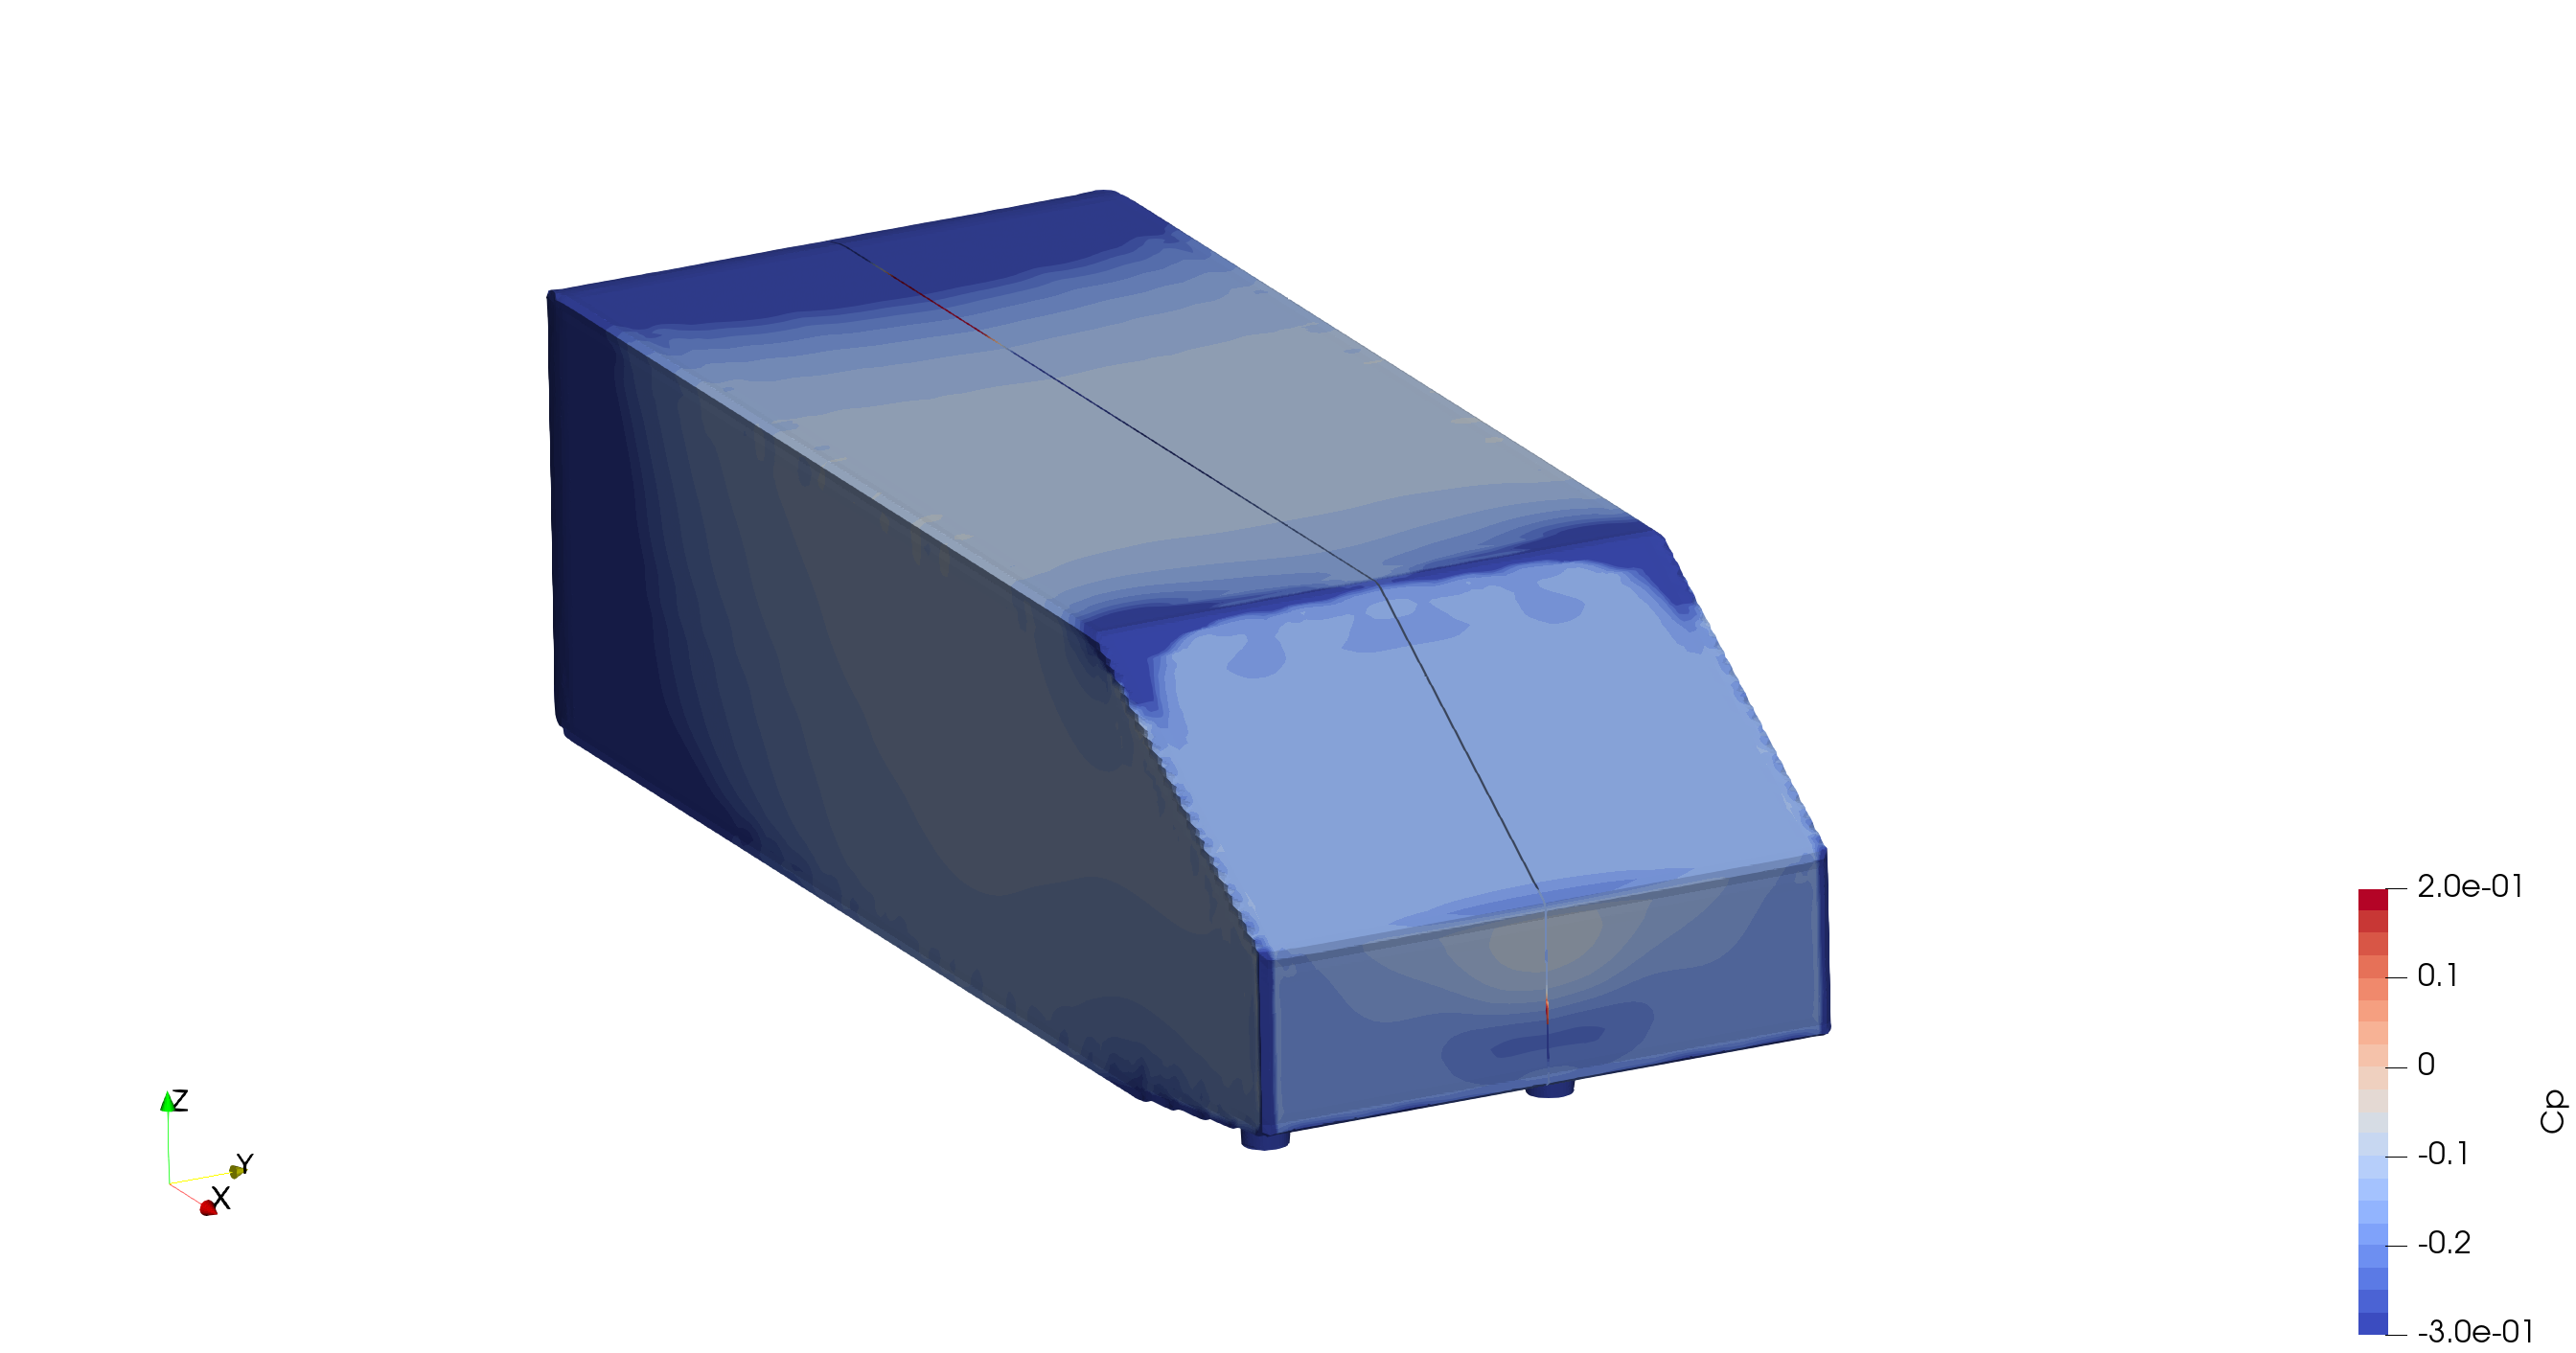
\includegraphics[width=\textwidth]{figures/cp_surface_L2}
    \caption{L2 mesh ($C_l = -0.327$)}
  \end{subfigure}
  \hfill
  \begin{subfigure}[b]{0.48\textwidth}
    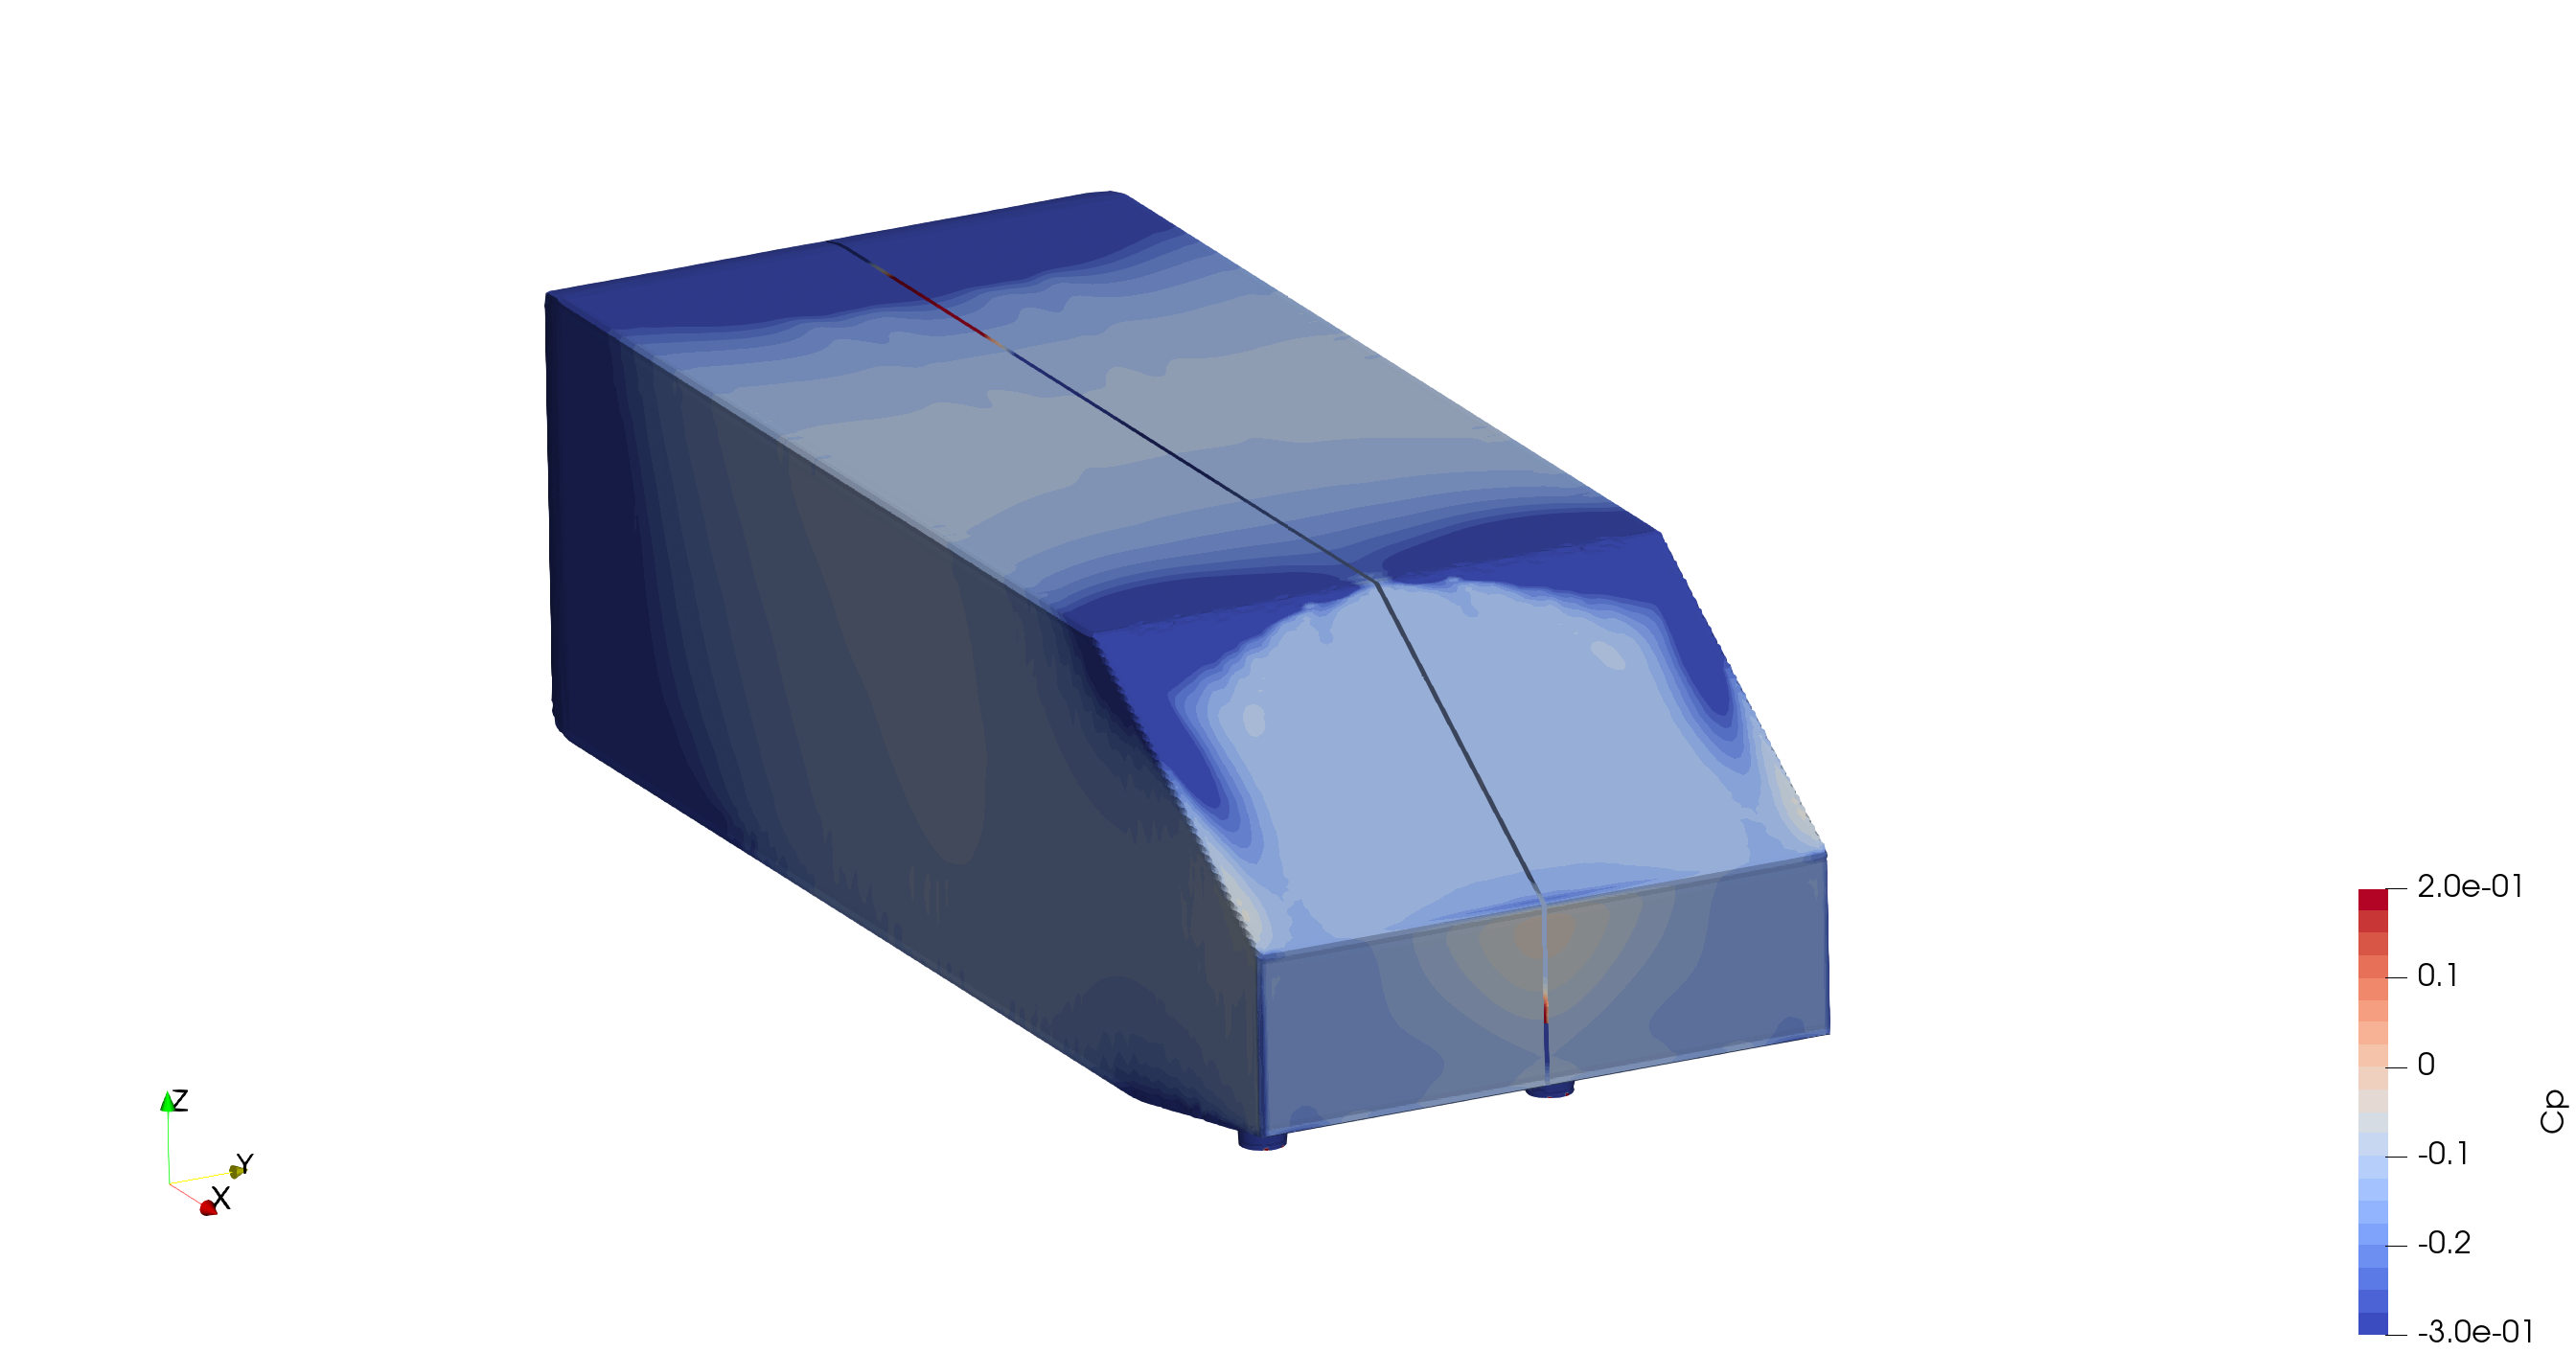
\includegraphics[width=\textwidth]{figures/cp_surface_L3}
    \caption{L3 mesh ($C_l = -0.167$)}
  \end{subfigure}
  \caption{Surface $C_p$ at the optimum design ($\alpha_\mathrm{slant}=32.5^\circ$, $\alpha_\mathrm{diff}=8.9^\circ$) on the L2 and L3 meshes. Colour range $-0.3$ to $+0.2$. The L2 mesh shows more uniform suction across the slant face; the L3 mesh distributes suction more strongly at the slant side edges with reduced central suction, consistent with earlier or more extensive boundary layer separation on the finer mesh.}
  \label{fig:cp_l2_l3}
\end{figure}

For the purposes of the initial single-fidelity campaign, all optimisation decisions were made on the consistent L2 RANS surrogate. The L3 result confirms that the optimum region ($\alpha_\mathrm{slant} \approx 32$--$34^\circ$) remains aerodynamically distinct from the low-slant minimum-drag regime. The absolute $C_d$ validation against experiment is performed at the baseline geometry (25° slant, no diffuser): L3 predicts $C_d = 0.325$ versus the Lienhart experimental value of $0.299$ ($+8.7\%$), consistent with kOmegaSST wall-function RANS over-prediction of separated-flow reattachment length (see \S\ref{sec:mesh_convergence}). The $C_d$ at the modified optimum geometry cannot be directly compared to the Lienhart value as the geometries differ. The $\Delta C_l = +0.160$ fidelity gap motivates the multi-fidelity correction described in \S\ref{sec:mf_results}.

% ----------------------------------------------------------------
\subsection{Multi-Fidelity Co-Kriging Results}
\label{sec:mf_results}

\subsubsection{L3 Anchor Results and Fidelity Correction}

Table~\ref{tab:l3_anchors_results} reports the 8 L3 anchor simulations used to train the additive correction GPs $\delta_{C_d}(\mathbf{x})$ and $\delta_{C_l}(\mathbf{x})$. Each anchor was solved on the L3 mesh using the same simpleFoam settings as the DoE (800 iterations, mean of last 200). The corrections $\delta = y_\mathrm{L3} - \hat{y}_\mathrm{L2}$ quantify the systematic fidelity gap at each location.

\begin{table}[h]
  \centering
  \caption{L3 anchor results and fidelity corrections. $\delta_{C_d} = C_{d,\mathrm{L3}} - \hat{C}_{d,\mathrm{L2}}$; $\delta_{C_l} = C_{l,\mathrm{L3}} - \hat{C}_{l,\mathrm{L2}}$, where $\hat{C}_{\cdot,\mathrm{L2}}$ is the L2 GP prediction at that location.}
  \label{tab:l3_anchors_results}
  \begin{tabular}{lccccccc}
    \toprule
    Case & $\alpha_s$ & $\alpha_d$ & $C_{d,\mathrm{L3}}$ & $C_{l,\mathrm{L3}}$ & $f_{\mathrm{L3}}$ & $\delta_{C_d}$ & $\delta_{C_l}$ \\
    \midrule
    l3\_anc\_000 & 32.5 &  8.9 & 0.3032 & $-$0.1670 & 0.2475 & $-$0.0113 & $+$0.1229 \\
    l3\_anc\_001 & 38.9 &  5.6 & 0.2921 & $-$0.1580 & 0.2395 & $-$0.0051 & $+$0.0118 \\
    l3\_anc\_002 & 15.8 &  2.1 & 0.2843 & $+$0.0031 & 0.2853 & $-$0.0117 & $-$0.0614 \\
    l3\_anc\_003 & 21.3 & 15.4 & 0.3061 & $+$0.1982 & 0.3722 & $-$0.0044 & $+$0.1672 \\
    l3\_anc\_004 & 27.6 &  9.2 & 0.3427 & $+$0.1846 & 0.4042 & $+$0.0271 & $+$0.0436 \\
    l3\_anc\_005 & 33.4 & 17.8 & 0.3978 & $+$0.3346 & 0.5093 & $-$0.0073 & $+$0.0816 \\
    l3\_anc\_006 & 36.7 &  3.8 & 0.2890 & $-$0.1016 & 0.2551 & $-$0.0125 & $+$0.0795 \\
    l3\_anc\_007 & 40.0 & 12.0 & 0.3039 & $-$0.1740 & 0.2459 & $-$0.0173 & $-$0.1137 \\
    \midrule
    \multicolumn{7}{l}{\footnotesize Mean $\delta_{C_d} = -0.0053$ (std $0.013$); mean $\delta_{C_l} = +0.042$ (std $0.087$)} \\
    \bottomrule
  \end{tabular}
\end{table}

\subsubsection{Co-Kriging Surrogate Validation}

Figure~\ref{fig:cokriging_validation} shows leave-one-out cross-validation of the co-Kriging HF surrogate at the 8 anchor locations. At each fold the correction GP is re-trained on 7 anchors and used to predict the held-out point. Leave-one-out MAEs are: $C_d$: 0.013, $C_l$: 0.103, $f_1$: 0.029. With only 8 anchor points the LOO error bars are wide; they are reported here as a qualitative sanity check rather than a claim of high accuracy.

\begin{figure}[h]
  \centering
  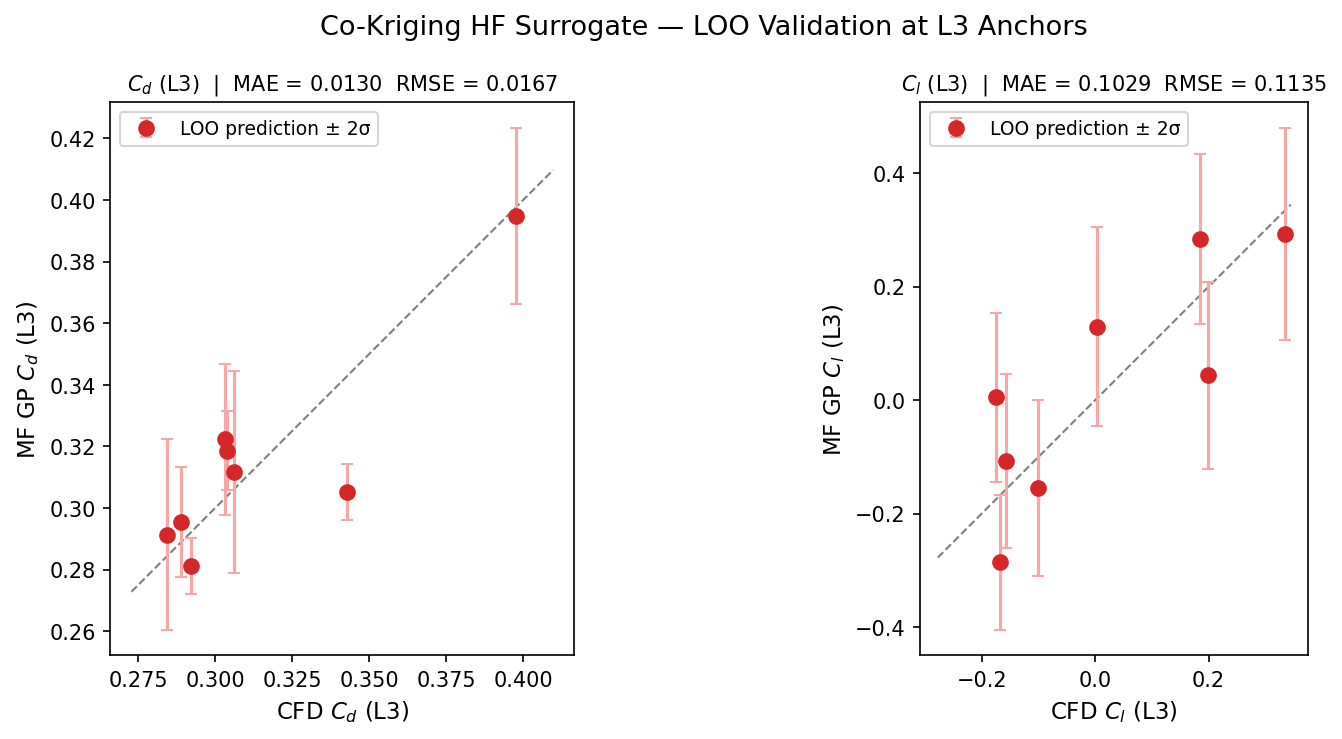
\includegraphics[width=0.85\textwidth]{figures/cokriging_validation}
  \caption{Co-Kriging HF surrogate leave-one-out validation at the 8 L3 anchors. Left: $C_d$. Right: $C_l$. Error bars show $\pm 2\sigma$ of the correction GP prediction. With 8 anchor points the correction GP is data-sparse; the uncertainty bands reflect this honestly.}
  \label{fig:cokriging_validation}
\end{figure}

\begin{figure}[h]
  \centering
  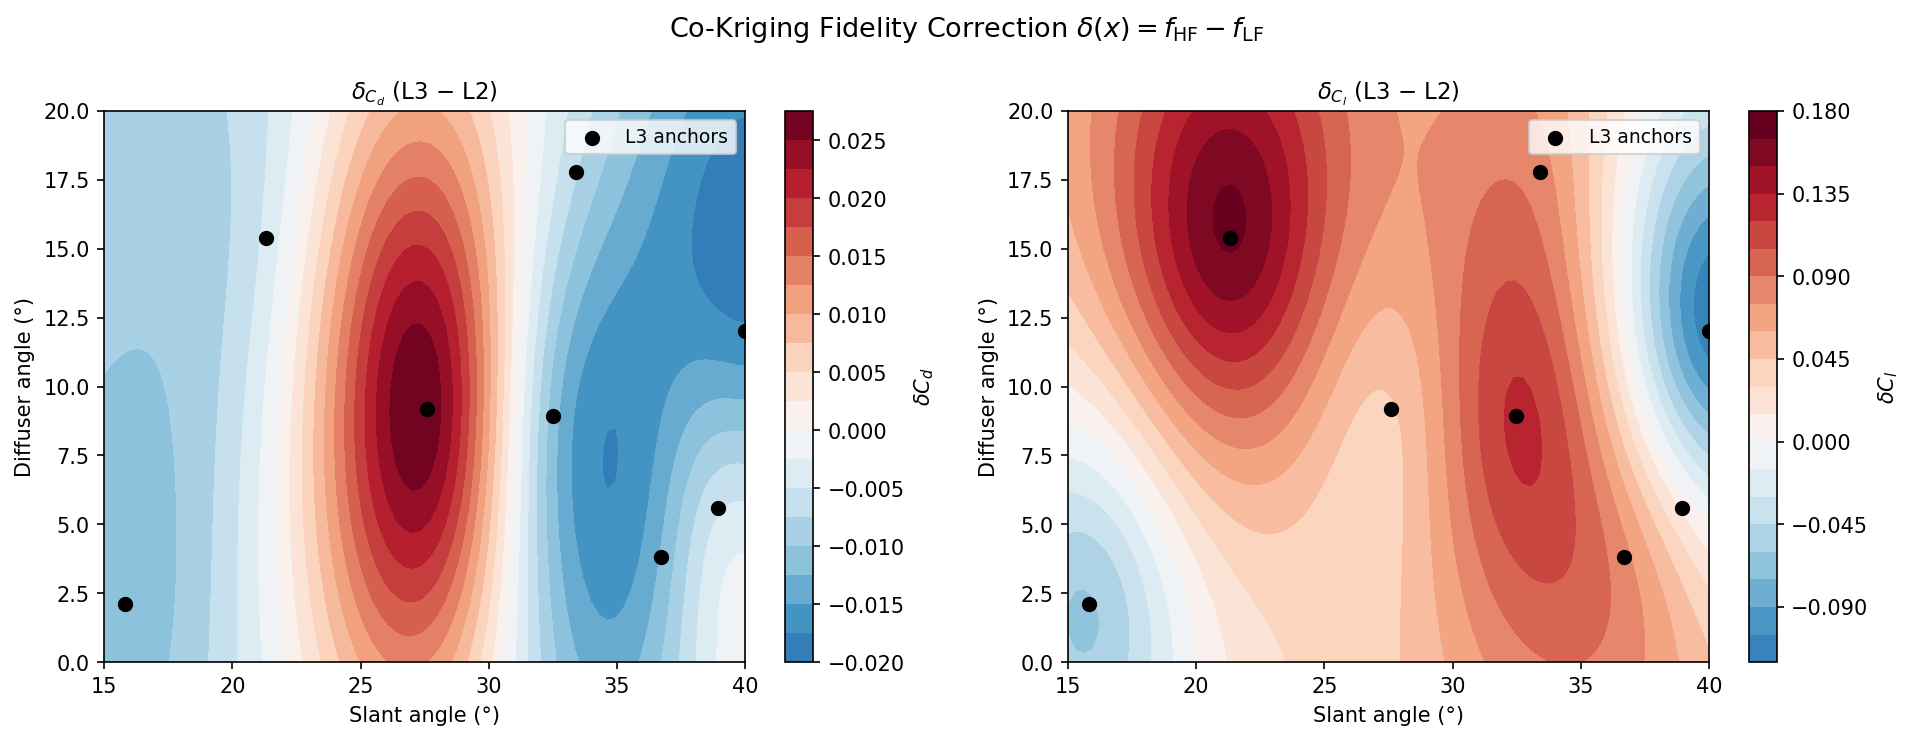
\includegraphics[width=0.85\textwidth]{figures/cokriging_correction}
  \caption{Correction response surfaces $\delta_{C_d}(\mathbf{x})$ and $\delta_{C_l}(\mathbf{x})$. Black dots mark the 8 L3 anchor locations. A spatially varying correction indicates that the fidelity gap is not a simple constant offset — the co-Kriging model accounts for this non-uniformity rather than applying a blanket bias correction.}
  \label{fig:cokriging_correction}
\end{figure}

\subsubsection{Multi-Fidelity Optimum}

\begin{table}[h]
  \centering
  \caption{Comparison of L2 single-fidelity and multi-fidelity co-Kriging optima.}
  \label{tab:mf_optimum}
  \begin{tabular}{lccccc}
    \toprule
    Surrogate & $\alpha_s^*$ (°) & $\alpha_d^*$ (°) & $C_d^*$ & $C_l^*$ & $f_1^*$ \\
    \midrule
    L2 RANS (single-fidelity)          & 32.5 &  8.9 & 0.319 & $-$0.327 & 0.210 \\
    MF co-Kriging (HF surrogate mean)  & 38.9 & 10.5 & $0.288\pm0.014$ & $-0.275\pm0.091$ & $0.196$ \\
    MF optimum verified (L3 CFD)       & 38.9 & 10.5 & 0.292 & $-$0.285 & \textbf{0.198} \\
    \bottomrule
  \end{tabular}
\end{table}

The MF co-Kriging surrogate predicted $f_1 = 0.1964$ at the identified optimum; the L3 CFD verification returned $f_1 = 0.1975$ — a $0.6\%$ surrogate error, well within the $\pm 2\sigma_\mathrm{HF}$ band. The verified MF optimum ($f_1 = 0.198$) represents a 5.7\% improvement over the L2 single-fidelity optimum ($f_1 = 0.210$) and a 20.2\% improvement over the L3 result at the original L2 optimum point ($f_1 = 0.248$). The $+4.9^\circ$ shift in diffuser angle reflects the co-Kriging correction increasing the predicted downforce at high slant in the HF surrogate — a correction that the L2 GP alone could not have captured.

The surrogate $C_l$ prediction error is $-0.009$ (within $0.1\sigma_\mathrm{HF}$), confirming that the correction GP's wide $\sigma_{C_l}$ was conservative: the actual HF $C_l$ is well-predicted at this location despite the large correction uncertainty seen in LOO validation.

Figure~\ref{fig:hf_response_surface} compares the L2 and MF optimum locations on the co-Kriging HF response surface.

\begin{figure}[h]
  \centering
  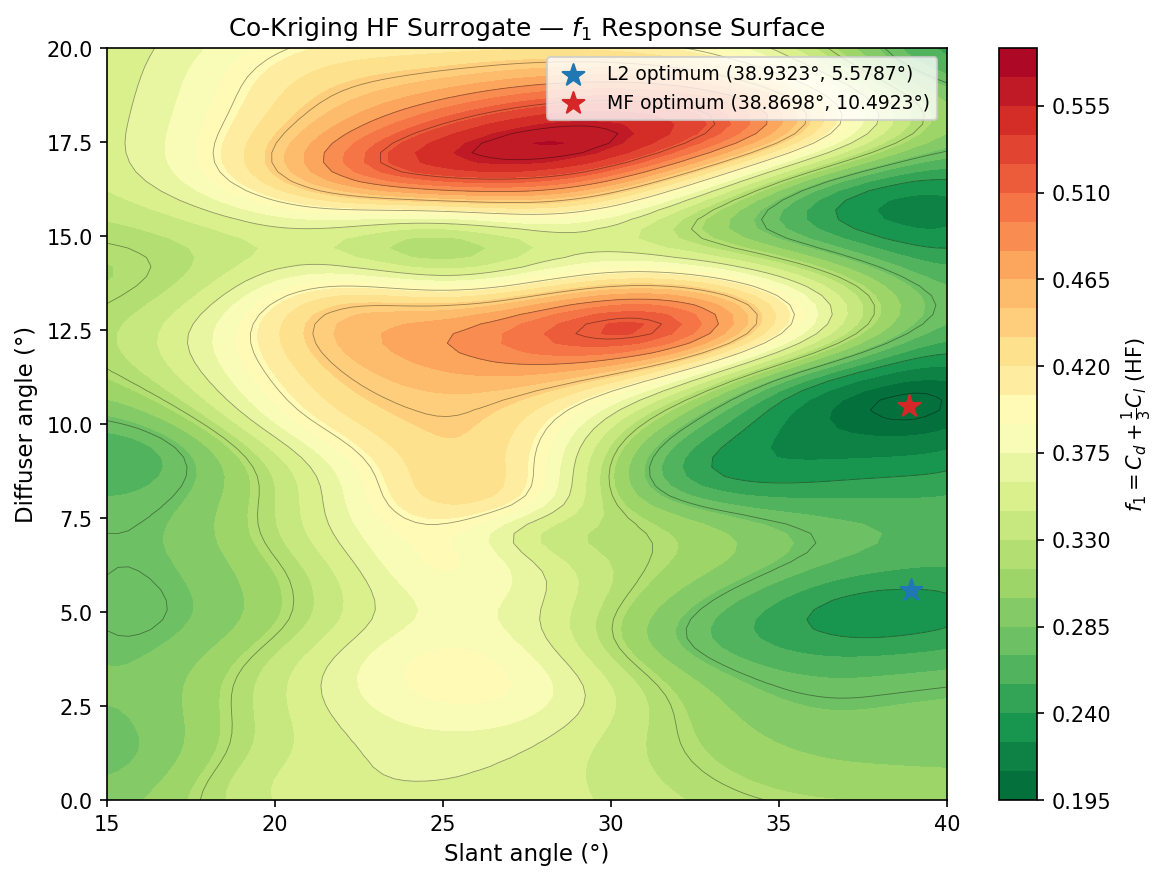
\includegraphics[width=0.85\textwidth]{figures/hf_response_surface}
  \caption{Co-Kriging HF $f_1$ response surface. The blue star marks the L2 single-fidelity optimum ($32.5^\circ/8.9^\circ$, $f_1=0.210$); the red star marks the verified MF co-Kriging optimum ($38.9^\circ/10.5^\circ$, $f_1=0.198$, L3 CFD). The $+4.9^\circ$ diffuser shift is driven by the HF correction increasing predicted downforce in the high-slant basin.}
  \label{fig:hf_response_surface}
\end{figure}

% ----------------------------------------------------------------
\subsection{Optimum Robustness: Basin Mapping and Critical-Angle Cliff}
\label{sec:stencil}

BO iteration~1 ($\alpha_\mathrm{slant}=35.7^\circ$, $\alpha_\mathrm{diff}=9.3^\circ$) returned $f_\mathrm{cfd}=0.642$ — a factor-of-three increase over the surrounding data. Post-hoc analysis confirmed this case is a genuine physics event rather than a solver failure: the mesh was of equivalent quality to converged cases (${\sim}435$K cells, solver reaching \texttt{End}) but the force coefficients exhibited a pseudo-time limit cycle ($\sigma_{C_d}=0.023$, $\sigma_{C_l}=0.097$ over the averaging window — see \S\ref{sec:des_statistics}). The reported training value is the mean of this oscillation. This indicates a bistable separated flow regime at this parameter setting: the steady RANS iterate does not converge to a fixed aerodynamic state, and the measured $f$ is not representative of either stable mode.

To verify that the verified MF optimum ($38.9^\circ$, $10.5^\circ$) sits in a basin rather than on a ledge adjacent to this cliff, six additional L3 RANS solves were performed in a stencil pattern (Table~\ref{tab:stencil_results}): one at the cliff point itself (L3 re-solve of the BO iter~1 geometry), one at the midpoint between cliff and optimum, and four forming a $\pm$plus-pattern around the optimum. The L3 re-solve at the cliff point ($35.7^\circ/9.3^\circ$) is itself instructive: the force history is well-converged ($\sigma_{C_d}=0.002$, compared to $\sigma_{C_d}=0.023$ for the equivalent L2 BO case), returning $f_1=0.215$. This confirms that the L2 training value of $f=0.642$ was a mesh-resolution artefact — the L2 mesh at this parameter setting produced a severe limit-cycle oscillation, but the L3 mesh resolves the flow to a stable, physically reasonable state.

The complete stencil reveals an asymmetric basin. The approach from the low-slant side passes through a local hump at $37.3^\circ$ (stn\_001, $f_1=0.234$) — the transition zone where flow is partially attached yet partially separated, yielding reduced downforce and elevated drag simultaneously. The surrogate predicts this approach as monotone ($\hat{f}_\mathrm{HF}=0.205$), missing the hump by $0.029$ in absolute $f_1$; this reflects the wider GP uncertainty in the transition band where the L2 training data were corrupted.

Moving away from the optimum in the $+\alpha_d$ and $+\alpha_s$ directions reveals sharp objective walls: $f_1$ rises from 0.198 to 0.258 ($+30\%$) at $\alpha_d=11.5^\circ$ and to 0.252 ($+27\%$) at $\alpha_s=39.5^\circ$. In both cases the penalty is driven by a collapse in downforce: $C_l$ deteriorates from $-0.285$ at the optimum to $-0.128$ (stn\_004) and $-0.145$ (stn\_005), indicating that pushing past the optimum loses the trailing edge separation pattern that generates the high-downforce state. The surrogate significantly under-predicts these walls ($\hat{f}_\mathrm{HF}=0.228$ and $0.198$ respectively), with the $+\alpha_s$ direction showing a 0.054 error — the surrogate extrapolates a near-flat landscape where CFD reveals a steep cliff. In the $-\alpha_d$ direction the basin degrades gently ($f_1=0.210$ at $9.5^\circ$, $+6\%$), in good surrogate agreement. The overall picture is a well-defined minimum with gentle slopes toward lower slant and lower diffuser, and sharp walls in the high-slant, high-diffuser quadrant.

\begin{table}[h]
  \centering
  \caption{L3 stencil results around the MF optimum and the critical-angle cliff. $\sigma_{C_d}$ is the standard deviation over the 200-iteration averaging window; oscillating cases ($\sigma_{C_d}>0.01$) are flagged. HF surrogate prediction $\hat{f}_\mathrm{HF}$ from the fitted co-Kriging model.}
  \label{tab:stencil_results}
  \begin{tabular}{lcccccc}
    \toprule
    Case & $\alpha_s$ & $\alpha_d$ & $C_d$ & $C_l$ & $f_1$ & $\hat{f}_\mathrm{HF}$ \\
    \midrule
    l3\_stn\_000 (cliff)      & 35.7 &  9.3 & 0.295 & $-$0.242 & 0.215 & 0.221 \\
    l3\_stn\_001              & 37.3 & 10.0 & 0.303 & $-$0.208 & 0.234 & 0.205 \\
    l3\_stn\_002              & 38.0 & 10.5 & 0.297 & $-$0.249 & 0.214 & 0.199 \\
    l3\_stn\_003 (opt $-1^\circ d$) & 38.9 &  9.5 & 0.288 & $-$0.235 & 0.210 & 0.215 \\
    l3\_stn\_004 (opt $+1^\circ d$) & 38.9 & 11.5 & 0.300 & $-$0.128 & 0.258 & 0.228 \\
    l3\_stn\_005 (opt $+0.6^\circ s$) & 39.5 & 10.5 & 0.300 & $-$0.145 & 0.252 & 0.198 \\
    \midrule
    MF optimum (verified)     & 38.9 & 10.5 & 0.292 & $-$0.285 & 0.198 & 0.196 \\
    \bottomrule
  \end{tabular}
\end{table}

% ----------------------------------------------------------------
\subsection{Slant-Angle Trend Validation}
\label{sec:slant_trend}

The absolute drag validation against experiment compares the L3 baseline geometry ($\alpha_\mathrm{slant}=25^\circ$, $\alpha_\mathrm{diff}=0^\circ$) to the Lienhart wind-tunnel reference ($C_d=0.299$): the L3 RANS predicts $C_d=0.325$, an 8.7\% over-prediction consistent with kOmegaSST in the separated Ahmed body regime. A stronger validation is to reproduce the characteristic Cd-vs-slant-angle \emph{trend} measured by Ahmed et al.~\cite{ahmed1984}: a rising $C_d$ up to the critical angle, followed by a sharp drop as the trailing vortex system breaks down and the slant separates fully.

Five L2 RANS solves at fixed $\alpha_\mathrm{diff}=0^\circ$ were run across the slant-angle range (Table~\ref{tab:slant_sweep}, Figure~\ref{fig:slant_trend}). The computed $C_d$ rises monotonically from $0.293$ at $12.5^\circ$ to $0.464$ at $35^\circ$. Qualitatively, the sub-critical rising trend ($12.5^\circ$--$30^\circ$) agrees with Ahmed (1984): both show a steady increase driven by growing C-pillar vortex strength. However, the super-critical $C_d$ drop observed experimentally at $35^\circ$ ($C_d \approx 0.300$) is absent in the simulation — the model predicts $C_d = 0.464$, a $55\%$ over-prediction at this angle.

This is a known limitation of steady kOmegaSST in the Ahmed body transition regime: the model delays the onset of full slant separation, effectively shifting the critical angle upward relative to experiment. The flow at $35^\circ$ remains in a partially-attached RANS state rather than the fully-separated state observed experimentally. This finding is consistent with the BO campaign results, where the surrogate identified $38.9^\circ$ as optimal — the RANS model continues to treat higher slant angles as beneficial because the critical-angle transition and associated $C_d$ reduction do not occur within the $15$--$40^\circ$ design space as modelled. The trend validation therefore confirms that the absolute performance predictions in the super-critical regime are unreliable, further motivating a URANS campaign in which the bistable transition is resolved time-accurately.

\begin{table}[h]
  \centering
  \caption{Computed $C_d$ vs slant angle at $\alpha_\mathrm{diff}=0^\circ$ (L2 mesh, kOmegaSST) compared to Ahmed (1984) experimental trend.}
  \label{tab:slant_sweep}
  \begin{tabular}{lcccc}
    \toprule
    $\alpha_\mathrm{slant}$ (°) & $C_d$ (L2 RANS) & $C_l$ (L2 RANS) & $C_d$ (Ahmed 1984\textsuperscript{a}) & Flow regime \\
    \midrule
    12.5 & 0.293 & $+$0.078 & ${\approx}$0.230 & Sub-critical, attached \\
    20.0 & 0.303 & $+$0.205 & ${\approx}$0.255 & Sub-critical, growing vortex \\
    25.0 & 0.326 & $+$0.074 & 0.299 \cite{lienhart2002} & Lienhart reference \\
    30.0 & 0.363 & $+$0.329 & ${\approx}$0.380 & Near-critical, max $C_d$ \\
    35.0 & \textbf{0.464} & $+$0.436 & ${\approx}$0.300 & \textbf{RANS fails: no transition} \\
    \bottomrule
    \multicolumn{5}{l}{\textsuperscript{a}Approximate values from Ahmed et al.~\cite{ahmed1984} Fig.~11; $\alpha_\mathrm{diff}=0^\circ$, no raised floor.}\\
  \end{tabular}
\end{table}

\begin{figure}[h]
  \centering
  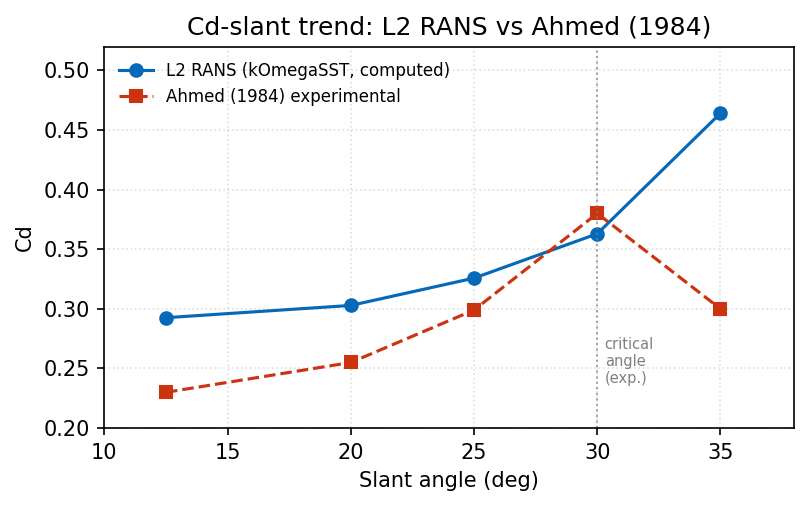
\includegraphics[width=0.65\textwidth]{../cfd_report/figures/slant_trend.png}
  \caption{$C_d$ vs slant angle: L2 RANS (circles) vs Ahmed (1984) experimental data (squares). The experimental critical-angle drop at ${\approx}30^\circ$ is absent in the RANS prediction; the model remains in a partially-attached regime up to $35^\circ$ and beyond.}
  \label{fig:slant_trend}
\end{figure}


